\section[Draw text as picture]{把文字绘制成图片}
字体排布的基本数据,如图\ref{fig:android_font_metric}及\ref{fig:android_font_metric_2}所示。

\begin{figure}
  \centering
  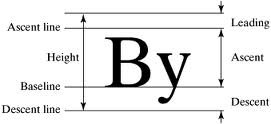
\includegraphics[width=.3\textwidth]{picturedir/font_metric.png}\\
  \caption{Font metric in Android}\label{fig:android_font_metric}
\end{figure}

\begin{figure}
  \centering
  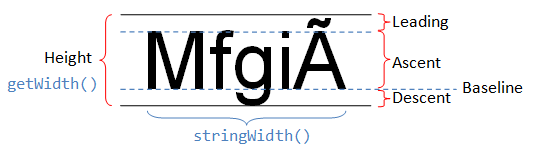
\includegraphics[width=.6\textwidth]{picturedir/font_metric_2.png}\\
  \caption{Font metric in Android}\label{fig:android_font_metric_2}
\end{figure}

\begin{javacode}
/**
 *  使用Paint类获取字体的metric信息。
 */
private Bitmap convertTextToBitmap(String text, float textSize, int textColor) {
  Paint paint = new Paint();
  paint.setTextSize(textSize);
  paint.setColor(textColor);
  paint.setTextAlign(Paint.Align.LEFT);
  
  int width = (int) (paint.measureText(text) + 0.5f);
  
  // Android中Y轴在屏幕上方,方向向下,所以ascent是负数,而descent是正数。
  float baseline = (int) (-paint.ascent() + 0.5f);
  int height = (int) (baseline + paint.descent() + 0.5f);
  
  Bitmap image = Bitmap.createBitmap(width, height, Bitmap.Config.ARGB_8888);
  Canvas canvas = new Canvas(image);
  canvas.drawText(text, 0, baseline, paint);
  return image;
}
\end{javacode}